A casual observation of the sea is enough to figure out that, the stronger the wind, the higher the height $H$ and length $L$
of the waves. From one location to another, it is also obvious that $L$ and $H$ change with the water body: a large lake can hold bigger waves than a pond, and waves in the 
Pacific, the largest water body on Earth, can reach close to 40 m high, with wavelengths above 600 m. Finally, within the same water body, the heights and lengths increase 
when moving downwind. The present chapter aims at providing a quantitative summary of observed wave properties, including useful empirical prediction formulae. These were the basis of
wave forecasting methods \citep[e.g.][]{Pierson&al.1955} before the advent of numerical models \citep{Gelci&al.1957}.

\section{Wind-sea growth}
A wide range of visual observations were systematically gathered by Sverdrup and Munk in 1941
in order to come up with a wave forecasting method for the U.S. Navy, faced with the delicate task of 
landing on the swell-battered beaches of Morocco. This work, initially classified, was only published as 
a landmark report after the war \citep{Sverdrup&Munk1947}. The miscelaneous observations were organized 
thanks to dimensional analysis with wave variables $H$ and $T$ expressed as a function of the wind speed 
$U_{10}$ as measured at 10 m above the sea surface, the fetch 
$X$, the duration $t$ over which of the wind has blown and the acceleration of gravity $g$. The fetch $X$ is the length 
of the region over which the waves have been generated. 

%%%%%%%%%%%%%%%%%%%%%%%%%%%%%%%%%%%%%%%%%%%%%%%%%%%%%%%%%%%%%%%%%%%%%%%%
\begin{figure}[htb]
\centerline{\includegraphics[width=0.8\textwidth]{FIGS_CH_FETCH/fetch_schematic.pdf}}
  \caption{Definition of fetch.}{Left: idealized conditions, Right: a real case 
  corresponding to the 2010 Xynthia Storm, which caused severe coastal flooding in France: the wind speed varies rapidly 
  in space and time, making it very difficult to define a fetch for an equivalent constant wind. The Xynthia storm crossed the bay of Biscay 
  in 6 hours going to the North-East, as a result the waves had little time to develop.} \label{fig:fetch}
\end{figure}
%%%%%%%%%%%%%%%%%%%%%%%%%%%%%%%%%%%%%%%%%%%%%%%%%%%%%%%%%%%%%%%%%%%%%%%%
In the open ocean, $X$ is not easy to define precisely, and it can 
be taken as an order of magnitude, in relation with a representative wind speed $U_{10}$: the region where winds are very high is typically smaller than the
region where winds are lower, so that the choice of the wind speed will modify the fetch. 

The use of $U_{10}$ as the variable representing the strength of the wind is also fairly arbitrary. 
Many studies have debated the possibly better choice of the friction velocity in the air, 
 $u_{\star a}=(\tau_a / \rho_a)^{1/2}$. %unfortunately, the scatter of wave parameters as a function  $u_{\star a}$ is almost as large as  when $U_{10}$ is used. 
Since wind speed measurements are usually converted to $U_{10}$ and more often measured than  $u_{\star a}$, it turns out to 
be more practical to use $U_{10}$. 
% NB: Analysis of Xynthia waves would be a good M1 / M2 topic. 

% LOGIC PROBLEM BELOW ... CF MARINE

In the most simple case, represented in figure \ref{fig:fetch}, 
a uniform wind speed blowing perpendicularly offshore from a straight shoreline. In such conditions 
Sverdrup and Munk found that the dimensionless wave energy  
\begin{equation}E^\star=E g^2 / U_{10}^4
\end{equation} and wave period
\begin{equation}
f_p^\star=f_p U_{10} / g
\end{equation}
%$\widetilde{E} = H^2 g^2 / U_{10}^4,$ 
% define E ...
 where $E$ and $f_p$ are the free surface elevation variance 
and the frequency of the elevation spectral peak, respectively, varies as a function of the dimensionless fetch
\begin{equation} X^\star=X g /
U_{10}^2 \end{equation} and duration
\begin{equation}
t^\star=t g/U_{10}.
\end{equation}
%A similar result was obtained for the  dimensionless wave period.  $1/f_p^\star= Tg / U_{10}$. 
Figure
(\ref{growthSHOWEX}) shows values measured at a time  $t^\star >
10^5$, for which the sea state does not depend on duration anymore. The figure also includes a comparison with 
the average measured values during other experiments \cite{Kahma&Calkoen1992,Kahma1981}.
%%%%%%%%%%%%%%%%%%%%%%%%%%%%%%%%%%%%%%%%%%%%%%%%%%%%%%%%%%%%%%%%%%%%%%%%
\begin{figure}[htb]
\centerline{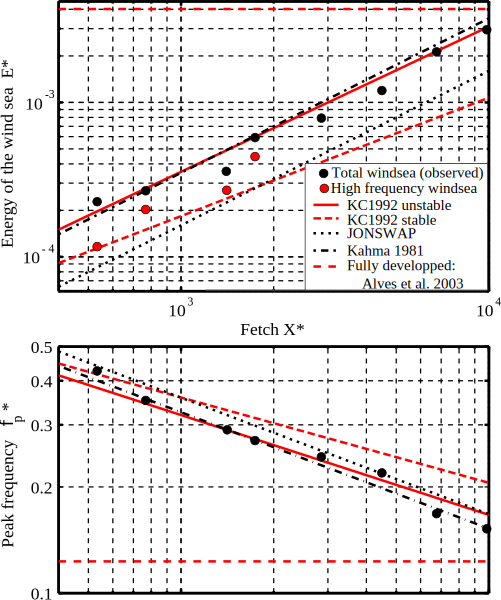
\includegraphics[width=0.6\textwidth]{FIGS_CH_FETCH/wave_growthSHOWEX_en.pdf}}
  \caption{Growth of waves with fetch, measured during  the Shoaling Waves Experiment (SHOWEX) in 1999, 
off the North Carolina Outer Banks. The wind is blowing at an angle of 70 degrees relative 
to the shoreline, which generates a double peak in the wind sea for the shortest fetches. Very close to shore, the 
high frequency part of the wind sea (in red) is in the wind direction, while an 'alongshore wind sea' (in black) grows to lower frequencies, 
in the direction of the largest available fetch. For comparison, several empirical growth curves 
are superimposed, as given by Kahma et Calkoen (1992), and Kahma (1981) from other datasets, and 
the expected 'full development' proposed by \cite{Pierson&Moskowitz1964}, as re-analysed by \cite{Alves&Banner2003}. \label{growthSHOWEX}}
\end{figure}
%%%%%%%%%%%%%%%%%%%%%%%%%%%%%%%%%%%%%%%%%%%%%%%%%%%%%%%%%%%%%%%%%%%%%%%%

%\subsection{La loi de Toba}
%Alors que les observations de $E^\star$ et $f_p^\star$ peuvent varier d'un
%facteur 2 pour une valeur de $X^\star$, Toba

\subsection{Full development and wave age}
For large fetches, the wave energy and peak frequency appear to tend to an asymptotic limit. 
This is very difficult to verify for moderate to strong winds, because the required non-dimensional fetch 
$X^\star_0=2.2 \times 10^4$ is already 220 km for $U_{10}= 10$ m/s. 
In practice we have very few observations for steady and uniform winds over a non-dimensional fetch larger than  $X^\star
> 10^4$. In search of such conditions, Pierson and Moskowitz
(1964\nocite{Pierson&Moskowitz1964}) have carefully selected 
55 records obtained from weather ships. From these measurements they estimated the asymptotic values  
\begin{equation}
E^\star=0.00402
 \end{equation}
 and
\begin{equation}
f_p^\star=0.123.
\end{equation}

The stage of development of waves, limited by fetch or duration, can be defined 
by the wave age, 
\begin{equation}
 A=C_p / U_{10}
\end{equation} where $C_p=2 \pi f_p/k_p$ is the phase speed at the peak of the spectrum. 
This parameter can be used to separate the wind sea, which is generated by the local wind and corresponds to 
young waves, with ages less than 1.2, and swell, for which the local wind has almost no effect, 
and which corresponds to older waves, with ages larger than 1.2. \cite{Donelan&al.1992} showed that 
the wave growth stops or at least becomes very slow, when  $C_p / U_{10} > 1.2$, confirming the analyses of \cite{Pierson&Moskowitz1964}. 
This means that, for a fully developped sea state, the dominant waves are propagating 20\% faster than the wind speed. 

\subsection{Fetch limitation}
The region where the wind is faster than a given value of  $U_{10}$ is always finite. This can limit the wave energy and peak frequency to a value 
lower than what would happen in a larger region. A practical important problem is the actual value reached by the wave height and peak period is 
such a limited area. With the non-dimensional fetch at full development $ X^\star_0 \simeq 2.2 \times 10^4$, all measurements lead to empirical 
wave growth formulae that are close to
\begin{eqnarray}
   C_p/U_{10}  & \simeq &  1.2  \left(\min
   \left\{\frac{X^\star}{X^\star_0},1\right\}\right)^{0.33},\label{ageElf}\\
   H_s  & \simeq &  0.26 \frac{U_{10}^2}{g}\left(\min
   \left\{\frac{X^\star}{X^\star_0},1\right\}\right)^{0.5}.\label{Hs_fetch}
\end{eqnarray}
We remember that in deep water, 
\begin{equation}
T_p = \frac{2 \pi C_p}{g},
\end{equation}
which yields $T_p$ from $C_p$.

The empirical growth laws (\ref{ageElf})--(\ref{Hs_fetch}) are a practical set of equations to 
obtain a quick estimate of the order of magnitude of the sea state, with heights within a factor two of the measurements, as shown in figure \ref{growthSHOWEX}.  
Many variants of thes equations have been published, with numerical values of the proportionality coefficients that may vary by a factor 2 \citep{Kahma&Calkoen1992}.
These differences are probably due, among other things, to the variations of the 
wind which is never exactly stationary nor uniform, and not exactly perpendicular to the shoreline... which is itself never quite straight and infinitely 
long. A careful analysis by \cite{Young1998} reveals that some of the differences between the different datasets may be due to differences between the air and sea 
temperature, which modify the properties of the turbulence in the atmospheric boundary layer. The details of how that impacts the wave growth is still 
not understood. One possible factor is that the wind tends to be less regular (more gusty) in unstable conditions when the water is warmer than the air. It is 
well understood that this increased gustiness can lead to higher waves for mature waves with $X^\star
> 10^4$, as shown by \cite{Abdalla&Cavaleri2002}. 
%%%%%%%%%%%%%%%%%%%%%%%%%%%%%%%%%%%%%%%%%%%%%%%%%%%%%%%%%%%%%%%%%%%%%%%%%%%%%%%%
\begin{figure}[htb]
\centerline{\includegraphics[width=\textwidth]{FIGS_CH_FETCH/fetch_time_lim_contours.pdf}}
 \caption{Estimation of significant wave height ($H_s$, contours) as a function of fetch and duration for the idealized case of an infinitely long coast 
with a wind blowing perpendicularly offshore at a speed $U_{10}=20$~m/s. In the left panel the estimate is given by a numerical integration of 
the wave action equation, defined in the next 
chapter, using parametrizations for the wind-wave growth and dissipation from \cite{Rascle&Ardhuin2013} and non-linear wave-wave interactions 
from \cite{Hasselmann&al.1985b} using the WAVEWATCH III model, with a third order numerical scheme \cite{Tolman1995b}. The right panel combines eq. 
(\ref{Hs_fetch}) and eq. (\ref{eq:time_limit}). Both give the time-limited growth for large fetches and the 
fetch-limited growth for large durations, with no more growth when waves reach full development at $H_s \simeq 10.8$~m. The dashed line is the same in both panels. 
In the left panel, the model gives a slow increase of the wave height even after the time limitation has been exceeded: this is because the infinitely long shoreline allows 
the growth of very oblique components that travel very long distances alongshore. That effect is not represented in the empirical formula of eq. (\ref{eq:time_limit}). 
It is a well documented effect for oblique fetches when the wind is not perpendicular to the coast \citep{Ardhuin&al.2007}, but there is no description of 
this phenomenon for winds perpendicular to shore. \label{fetch_time}}
\end{figure}
%%%%%%%%%%%%%%%%%%%%%%%%%%%%%%%%%%%%%%%%%%%%%%%%%%%%%%%%%%%%%%%%%%%%%%%%%%%%%%%%%

\subsection{Time limitation}
If the wind has started to blow only a short time ago, with $t^\star < 10^5$, the sea state parameters 
can be estimated, replacing $X^\star$ with
\begin{equation}
X^\prime = (t^\star/70)^{1.3}. \label{eq:time_limit}
\end{equation} 

\subsection{Double limitation}
In practice, the sea state is often limited by both time and fetch. 
The sea state parameters are then given the lowest of the two values for $H_s$ and $C_p/U_{10}$ 
between the one obtained with $X^\star$ and the one obtained with $X^\prime$ \citep[see][]{CERC1977}. 
For an alternative estimation, one may read \cite{Hwang&Wang2004}. This double limitation is illustrated by figure \ref{fetch_time}.



\section{Swell}
So far we have only discussed the wind sea, which is related to the local wind. However,  
the sea state often contains an important swell contribution, which are waves radiating away from their area of generation. We can define swells as the waves for which the source 
of energy from the wind is zero or negative, in practice it corresponds to waves travelling at a phase speed $C$ faster than the wind speed $U_{10}$, or at angle relative 
to the wind $\theta_w - \theta_u$ such that $U \cos(\theta_w-\theta_u) < C$. This definition is often extended to allow the peak of a fully developped wind sea, which can 
travel at a phase speed of 1.2 $U_{10}$, to be classified as wind sea. This extension is equivalent to adding the source of energy from the nonlinear wave-wave interactions to 
the source of energy from the wind in order to separate wind seas and swell. Because the wind is neither steady nor uniform the boundary between wind sea and swell is rather 
fuzzy. 

Swells is most important in large oceanic basins, in particular near their eastern boundary as the dominant winds generally blow from west to east where it can account for 
more than 90\% of the wave energy \citep[e.g.][]{Chen&al.2002}. The swell is the part of the sea state that cannot be amplified 
by the local wind because they are too fast, or travel at an angle too oblique to the local wind. 
This swell can be composed of distinct individual swells, travelling in different directions and 
with different dominant frequencies, these swells are the result of the evolution of 
wind seas that propagate out of their generation area. 
Swells, when they exist, generally have longer periods than the wind sea because short waves are rapidly dissipated away from their generation area. They are thus the result of storm conditions, with winds strong enough to generate large period waves, as given by eq. \ref{ageElf}. The stronger and larger the storm, the longer the swell period. 
%%%%%%%%%%%%%%%%%%%%%%%%%%%%%%%%%%%%%%%%%%%%%%%%%%%%%%%%%%%%%%%%%%%%%%%%%%%%%%%%
\begin{figure}[htb]
\centerline{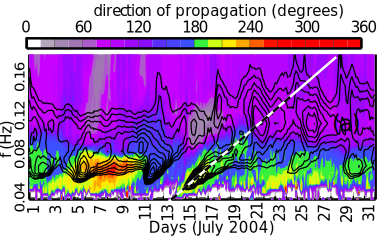
\includegraphics[width=0.8\textwidth]{FIGS_CH_FETCH/SWAO_nature_figS1_en.pdf}}
 \caption{Example of the evolution of wave energy and mean direction as a function of frequency
and time, over one month, measured at the Christmas Island buoy (Kiritimati, Kiribati), 
in the middle of the Pacific. Contour values equally spaced between 
0.1 and 1.4 correspond to the logarithm of the spectral density $E(f)$, colors 
correspond to the mean direction for each frequency. The oblique dashed line 
from 15 July at 0.05 Hz to 18 July at 0.8 Hz correspond to eq. (\ref{prev lin1}) 
with a distance $R \alpha= 6100$~km between storm and observation point. 
The intersection between this line and the axis $f=0$ gives the date of the storm: July 9, 
when a severe storm was indeed present south of New Zeland. \citep[taken from][]{Collard&al.2009}.\label{ridges}}
\end{figure}
%%%%%%%%%%%%%%%%%%%%%%%%%%%%%%%%%%%%%%%%%%%%%%%%%%%%%%%%%%%%%%%%%%%%%%%%%%%%%%%%%

Modern swell studies started during the colonial war between France and Morocco in 1906. In the absence of safe harbors on the atlantic coast of Morocco, the disembarkment of troops and supplies used small shuttle boats that could be destroyed by heavy swells. Such an event made the harbor of Casablanca unavailable for several months. 
Swell forecasting for Morocco became a an important matter, and the first method was based on 
the propagation of swells from the mid-atlantic Azores Islands where visual observations were made several times a day \citep{Gain1918}. 
This method was used in the swell forecasting office of Casablanca in the early 1920s \citep{Montagne1922}, where the first modern numerical wave models were invented \citep{Gelci&al.1957}. 

In the Pacific or Indian oceans, it is very common to find at the same time and place 
 several swells coming from distinct storms (e.g. Figure \ref{fig:Hawaii_spectrum}), that may have happened 10,000 km away and a week before \citep{Darbyshire1957, Munk&al.1963}. 
Owing to the large distances travelled by swells, the sphericity of the Earth must be taken into account. The re-derivation of linear wave theory in that case 
shows that the swell that propagated along a straight line on a flat ocean, now travel on the shortest path on the sphere, which are the great circles:  
the circles that have their centers at the center of the Earth, such as the meridians. 

The height and period of swells depend on the height and period of waves in the strom, and the propagation distance outside of the storm. Storms generate waves with a wide range of periods up to about 1.2 times the peak period $T_p$. This mixture of waves `disperses', and because the group speed $C_g=g T/(4 \pi)$  in deep water, is a function of the period $T$, 
the largest period swell arrive first, followed by shorter swells. 
At very large distances, the storm from which the swell radiates can be considered a point in 
space and time. The evolution of the swell peak period at a remote observation position follows, 
\begin{equation}
T_{\mathrm{ps}} (t) = \frac{4\pi R \alpha }{g(t-t_0)},
\label{prev lin1}
\end{equation}
where $R$ is the Earth radius, $t_0$ is the time of the storm, and $\alpha$ is the spherical distance, i.e. the angle -- in radians -- at the center of the Earth between the storm and the observation point. This relationship very well verified, as shown in figure \ref{ridges}.


Swell heights decrease during propagation due 
to the dispersion from the source, and also due to dissipation. Dispersion is the main effect for swell periods larger than 12 s, 
and corresponds to a stretching of the wave fronts in the direction perpendicular to propagation, just like circles becoming larger 
away from a stone dropped in a pond. There is also a stretching of the wave train in the propagation direction due to the different group 
speeds, the longer wave periods contribute to a longer wave train away from the storm, while the shorter wave periods are travelling 
slower behind. This spatial spreading of the swell field is illustrated with numerical model results in 
figure \ref{reconst_champ}, taken from \cite{Delpey&al.2010}. 
%%%%%%%%%%%%%%%%%%%%%%%%%%%%%%%%%%%%%%%%%%%%%%%%%%%%%%%%%%%%%%%%%%%%%%%%%%%%%%%%%%%%%%
\begin{figure}[htb]
\centerline{\includegraphics[width=0.6\textwidth]{FIGS_CH_FETCH/partition_globes_small.pdf}}
 \caption{Swell radiated from a storm.}{(a,b,c) peak periods of the swell $T_{ps}$ and (d,e,f) significant swell heights  $H_{ss}$ 
from a realistic numerical model of the storm of February 24, 2004, centered at (160$^{\circ}$ E, 42$^{\circ}$ N). 
The maps correspond to  February 27th (top) 
 March 1st (middle) and March 6th (bas) at 00h UTC, which is 3, 6 and 9 days after the storm \citep[reproduced from][]{Delpey&al.2010}.\label{reconst_champ} }
\end{figure}
%%%%%%%%%%%%%%%%%%%%%%%%%%%%%%%%%%%%%%%%%%%%%%%%%%%%%%%%%%%%%%%%%%%%%%%%%%%%%%%%%%%%%%
Neglecting dissipation effects, and for distances of the order of 4000 km or more from the storm center, 
the decrease in swell height following the peak in space and time is given by 
\begin{equation}
H_{ss} (\alpha) = H_{ss} (\alpha_0)  \sqrt{\frac{\alpha_0  \sin \alpha_0}{\alpha \sin \alpha}}.
\label{swell_asymptote}
\end{equation}
In practice, the height is further reduced by islands and continents 
where it breaks and dissipates on the shore. Dissipation in deep water is locally weak but can add up to a significant effect 
over long propagation distances \citep{Ardhuin&al.2009b}. Even with these effects, it is possible to record swells coming from the 
antipodes \citep[e.g.][]{Munk&al.1963}. 
 

\section{Frequency spectra}
\subsection{The early days}
The first measurements of wave spectra from time series were performed in 1944, as part of the efforts of Group W at the British Admiralty, 
after the amphibious assault on Normandy  \citep[][]{Barber&al.1946,Ursell1999}. These records, and the many others that followed, 
revealed that for frequencies above the spectral peak, the decrease in energy takes always the same form. \cite{Phillips1958}
 introduced the idea of an  equilibrium region for
$f>f_p$, and proposed that gravity was the only determining factor for that part of the spectrum which was controlled by wave breaking.  
Dimensional analysis leads to the shape 
\begin{equation}
   E(\sigma)=\alpha_P g^2 \sigma^{-5} \quad \mathrm{or} \quad E(f)=\alpha_P \left(2\pi\right)^{-4} g^2 f^{-5},
\end{equation}
where $\alpha_P\approx 0.008$ is now called Phillips' constant. The non-dimensional energy $E(\sigma) \sigma^{5}/g^2$ is constant
in this model: the surface is thus fractal without any particular scale. In other words, these waves are self-similar and have all the same shape, whether they are large or small. 
%%%%%%%%%%%%%%%%%%%%%%%%%%%%%%%%%%%%%%%%%%%%%%%%%%%%%%%%%%%%%%%%%%%%%%%%%%%%%%%%%%%%%%%%%%%%
\begin{figure}[!hbt]
\centerline{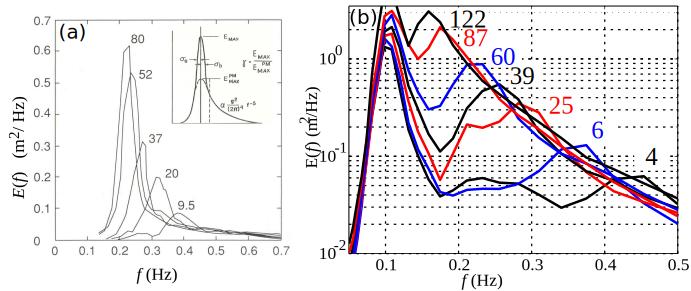
\includegraphics[width=\textwidth]{FIGS_CH_FETCH/overshoot_JONSWAP_SHOWEX.pdf}}
  \caption{Evolution of the wave spectrum with fetch.}{(a) measured spectra on September 15, 1968 at 11h
  during JONSWAP, with, inset, the proposed parameters for the JONSWAP spectrum. Numbers indicate the fetch in kilometers. (b) spectra measured on November 3rd, 1999, averaged from 13h to 17h during SHOWEX, 
using Datawell Mark III waverider buoys. 
Note that the scale is logarithmic. In the SHOWEX case, the wind speed is 10 m/s, 20 degrees from the shore-normal. The peak around $f=0.1$~Hz
  corresponds to swell arriving from the Atlantic, against the wind. The instrument at the shortest fetch 
reveals two peaks in the wind sea, at 0.25 and 0.45 Hz. The analysis of wave directions, not shown here, show that the first peak is propagating 
alongshore, and the second is in the 
wind direction. The existence of the first peak is due to the oblique 20$^\circ$ angle between the wind and the shore-normal.}
\label{fig_overshoot}
\end{figure}
%%%%%%%%%%%%%%%%%%%%%%%%%%%%%%%%%%%%%%%%%%%%%%%%%%%%%%%%%%%%%%%%%%%%%%%%%%%%%%%%%%%%%%%%%%%%
These ideas were also developed by \cite{Kitaigorodskii1962}, and  led \cite{Pierson&Moskowitz1964} to propose an empirical 
shape for the full spectrum, based on fully developed sea states, 
\begin{equation}
   E(f)=E_{PM}(f)=\alpha_{P} g^2 \left(2\pi\right)^{-4} f^{-5} \exp\left[-\frac{5}{4}
   \left(\frac{f}{f_p}\right)^{-4}\right].
\end{equation}
At short fetch, it was soon realized that spectral shapes could be significantly different. 
The peak is particularly narrower for young sea states. Also, the values of the spectral density $E(f)$ for a given frequency $f$
can be larger than those found for old seas: this overshoot of the spectral peak was first discussed by \cite{Barnett&Sutherland1968}, 
and further investigated during the 1968-1969 Joint North
Sea Wave Project \citep[JONSWAP, see][]{JONSWAP},
figure \ref{fig_overshoot}).

Based on these observations, a `peak enhancement' was added to the Pierson-Moskowitz (PM) shape, 
\begin{equation}
   E(f)=E_{PM}(f) \gamma^{\exp\left[\frac{-\left(f-f_p\right)^2}{2 \sigma_{A/B}^2
   f_p^2}\right]}. \label{SpectreJONSWAP}
\end{equation}
This may look a bit complex, but each parameter plays a fairly clear role, illustrated in figure \ref{fig_overshoot}.a. 
$\gamma \simeq 3.3$ is the `peak enhancement-factor', if equal to 1 then the spectrum is a PM spectrum,  $\sigma_{A/B}$ 
is the relative width over which this enhancement applies. It was found that  $\sigma_{A} \simeq 0.07$
if $f<f_p$ and $\sigma_{B} \simeq 0.09$ otherwise. Using (\ref{SpectreJONSWAP}) and (\ref{ageElf}) one can estimate 
 $C_p$ and $f_p=g/(C_p 2 \pi)$ as a function of the wind speed. This gives the average spectral shape measured 
in the North Sea during JONSWAP. 

\subsection{The modern era}
More recent obvservations, starting with \cite{Toba1973}, have shown that, at frequencies between 
$f_p$ and $3 f_p$, the spectrum was not following  $f^{-5}$ but  $f^{-4}$. This shape can be obtained 
by including the wind speed or friction velocity in the dimensional analysis, it also corresponds to a 
constant flux of energy towards high frequencies due to the non-linear wave-wave interactions. In passing, we can see 
that it is always easy to find a theory for anything after the observations have been made. 
This $f^{-4}$ decrease near the spectral peak is particularly well verified by the wave gauge array data of \cite{Donelan&al.1985}, 
which was one of the first clean measurements of the spectrum in both frequency and directions. \cite{Donelan&al.1985} also proposed 
a spectral shape that reconciles the peak enhancement of the JONSWAP data with the mature wave spectral shape of \cite{Pierson&Moskowitz1964}. 
The adjustment given here in eq. (\ref{ageElf}) is an adaptation by \cite{Elfouhaily&al.1997}, giving the proper asymptotes for wave energies and periods. 
Further analysis by \cite{Long&Resio2007} have shown that there is in general a transition from  $f^{-4}$ at frequencies above the windsea peak  to  $f^{-5}$ at higher frequencies, and the 
frequency where this transition occurs appears to be a function of wave age. 

This discussion of the detailed shape of the wave spectrum at frequencies beyond $2 f_p$ may sound unimportant because it affects a very small fraction of the wave energy.
However, that part of the spectrum supports most of the energy flux from the wind to the waves, and thus defines the roughness of the sea, and thus the growth rate due to the wind for
the entire spectrum. Also, these short waves dominate the surface slopes, which strongly affect ocean remotely sensed properties such as sea level, surface salinity and wind speed 
and direction. Measurements of the sun reflection by the ocean performed by \cite{Cox&Munk1954} give a very good estimate of the mean square slope (mss),
\begin{equation}
   \mathrm{mss}=\int \left(k_x^2+ k_y^2 \right) E(k_x,k_y) {\mathrm d} k_x {\mathrm d} k_y \simeq
   \int \frac{(2 \pi f)^4}{g^2} E(f) {\mathrm d} f, \label{eq:mss_int}
\end{equation}
where the second equality uses the linear wave approximation. In order to have a finite value of the mss, 
$E(f)$ must decrease faster than $f^{-5}$ towards the high frequencies. 
\cite{Elfouhaily&al.1997} and \cite{Kudryavtsev&al.1999} have used this argument and detailed remote sensing data to propose a parametric 
shape of the wave spectrum that is a function of wind speed and wave age, and includes a strong decrease for  $k> 10 k_p$, 
taking also into account the effect of surface tension \citep[see also][]{Dulov&Kosnik2009,Yurovskaya&al.2013}.
A few proposed parametric spectral shapes for gravity waves are compared in figure \ref{spectra_comp}. In practice there is a very strong variability 
of the observed specta around these average shapes due to spatial and temporal variations in wind speed and direction.
It should also be noted that for $f > 4 f_p$ there can be a dominant contribution of non-linearities, as revealed in stereo-video imagery (see figure \ref{fig:kxky} in 
the preceding chapter).

%%%%%%%%%%%%%%%%%%%%%%%%%%%%%%%%%%%%%%%%%%%%%%
\begin{figure}[htb]
\centerline{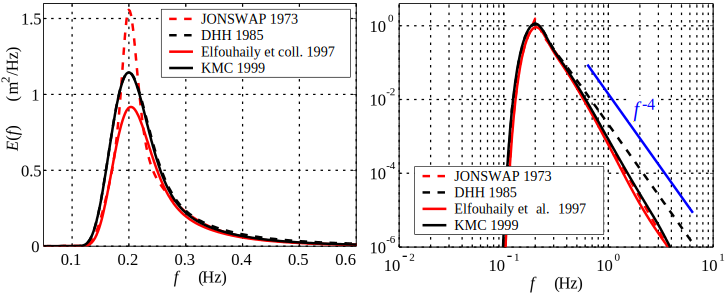
\includegraphics[width=\textwidth]{FIGS_CH_FETCH/Spec_comp50km_linlog_en.pdf}}
%\vspace{3.64in}
  \caption{Example of proposed parametric wave spectrum shapes, for $U_{10}=10$~m~s$^{-1}$ et $X=50$~km. Left: using a linear scale and 
right, the same spectra with a logarithmic scale. The slope of the curves in log scale gives the power  $n$ of the 
  dependance  $E(f) \propto f^{-n}$. Note the transition from
  $n=4$ for $f< 2 f_p$ to $n>5$ at higher frequencies, broadly consistent with the analysis of \cite{Long&Resio2007}. 
  We have extended here the \cite{Donelan&al.1985} spectrum beyond its range of validity, namely for $f>3 f_p$, in order 
to better visualize its  $f^{-4}$ decay.}
\label{spectra_comp}
\end{figure}
%%%%%%%%%%%%%%%%%%%%%%%%%%%%%%%%%%%%%%%%%%%%%%%

\section{Directional spectra} 
\subsection{Early parameterizations}
The distribution of wave energy as a function of directions, is still very much debated because of the 
difficulty of measuring details of that distribution. Indeed, a wave buoy only measured 5 parameters for each direction \citep[e.g.][]{Kuik&al.1988}, and even 
ADCP systems are generally too noisy to go beyond the mean direction and possibly spreading at each frequency \citep{Herbers&Lentz2010}. 
There are, however, important constraints on the high frequency directional distribution, with a surface slope variance which is almost the same in the downwind and 
crosswind directions. 

The frequency-direction spectrum $E(f,\theta)$ is often decomposed into a frequency spectrum and a 
normalized directional distribution 
\begin{equation}
   E(f,\theta)=E(f)S(f,\theta)
\end{equation}
with the normalization
\begin{equation}
   \int_0^{2\pi} S(f,\theta) {\mathrm d}\theta=1.
\end{equation}

The first parameterizations of $S(f,\theta)$ used the fact that $S$ is a periodic function 
and that buoys can provide the first terms in its Fourier decomposition, 
\begin{equation}
S(f,\theta)=\frac{1}{2\pi} + a_1(f) \cos(\theta) + b_1(f) \sin(\theta) + ... 
\end{equation}
This was soon abandonned because $S$ can be negative for some directions if the series is truncated. \cite{Longuet-Higgins&al.1963} proposed 
another distribution that is always positive  
\begin{equation}
   S(f,\theta)=\cos^{2s}\left((\theta-\theta_m)/2\right),
\end{equation}
which is symmetric about the direction of the maximum $\theta_m$, and narrower for larger $s$. This shape is still widely used, 
although $s$ cannot be readily measured, whereas the directional spreading  $\sigma_\theta$ (defined in 
chapter \ref{ch2}), is directly related to co-spectra of measured displacements or velocities. 
The width of the directional spectrum is generally minimum at the spectral peak, and increases towards both higher 
and lower frequencies.  The mean direction, even for the wind sea, can differ significantly from the wind direction, 
in particular at short fetch (see figure
\ref{fig_SHOWEX_dir}).

Among other proposed forms, the one by \cite{Donelan&al.1985} is based on theoretical solutions for non-linear wave groups,
\begin{equation}
   S(f,\theta) \propto \frac{1}{\cosh^2\left[\beta \left(\theta-\theta_m\right)\right]}
\end{equation}
and observations suggest $\beta = 2.44 (f/0.95 f_p)^{1.3}$ for $0.56<f/f_p < 0.95$ and
$\beta = 2.44 (f/0.95 f_p)^{-1.3}$ for $0.95<f/f_p < 1.6$. 
%From stereo-photographs, which cannot 
%resolve a 180 degree ambiguity in the propagation direction, 
%\cite{Banner1990} proposed $\beta =
%10^{-0.4+0.8393 \exp\left[-0.567 \ln\left(f/f_p\right)^2\right]}$
%for $f/f_p > 1.6$. 
That particular shape has been used for the estimation of the wind direction from HF radar data because they have non-zero values 
in the direction opposite to the wind direction, consistent with radar data. Unfortunately they still have a single maximum. 
%%%%%%%%%%%%%%%%%%%%%%%%%%%%%%%%%%%%%%%%%%%%%%%%%%%%%%%%%%%%%%%%%
\begin{figure}[htb]
\centerline{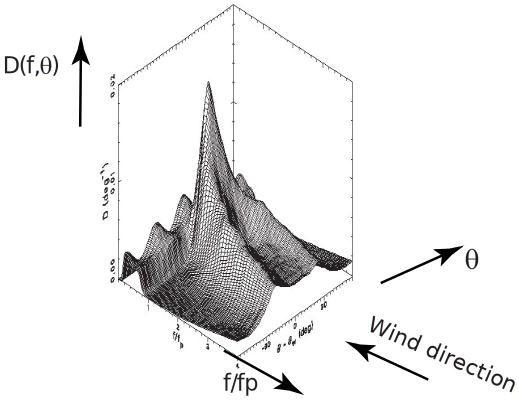
\includegraphics[width=0.7\textwidth]{FIGS_CH_FETCH/bimodal_en.pdf}}
%\vspace{3.64in}
  \caption{Average spectral distribution measured in Currituck sound for $U_{10} > 7$~m~s$^{-1}$ (From Long and Resio 2007).}
\label{bimodal}
\end{figure}
%%%%%%%%%%%%%%%%%%%%%%%%%%%%%%%%%%%%%%%%%%%%%%%%%%%%%%%%%%%%%%%%%

\subsection{Bimodality of the directional spectrum}
Indeed, detailed observations using arrays \citep{Young&al.1995,Long&Resio2007} or surface mapping systems with radar or optical imagery 
\citep{Hwang&al.2000b,Romero&Melville2010,Leckler&al.2015} have clearly revealed that for  $f > f_p$ the wind sea generally has two peaks 
on either side of the wind direction, as shown in figure 
\ref{fig:kxky} and \ref{bimodal}. Such a distribution is called bimodal. For frequencies $f>3f_p$ these peaks are 60 to 80 degrees 
away from the wind direction, at least for young waves ($C_p/U_{10} < 1/3$). 
There is no simple parametric form for these bimodal spectra, and their general shape for more mature waves is not established. 
Also, numerical models have a hard time reproducing clearly bimodal spectra, as discussed by \cite{Alves&Banner2003}. In general, for the dominant waves, we only have a good knowledge of the mean direction and directional spreading. 
One example of these two parameters is shown in figure \ref{fig_SHOWEX_dir}).
%%%%%%%%%%%%%%%%%%%%%%%%%%%%%%%%%%%%%%%%%%%%%%%%%%%%%%%%%%%%%%%%%
\begin{figure}[htb]
\centerline{\includegraphics[width=0.7\textwidth]{FIGS_CH_FETCH/showex_spectra_dir.pdf}}
%\vspace{3.64in}
  \caption{Example of measured directional parameters}{Measurements during SHOWEX on November 3rd 2003, in presence of a 1 m swell opposing 
the wind sea. The wind direction is from 270$^\circ$ and the shoreline faces 70$^\circ$. 
The different wave systems are clearly separated by a local maximum of the directional spreading 
  $\sigma_\theta$}.
\label{fig_SHOWEX_dir}
\end{figure}
%%%%%%%%%%%%%%%%%%%%%%%%%%%%%%%%%%%%%%%%%%%%%%%%%%%%%%%%%%%%%%%%%

As a result, applications that require a detailed knowledge of the directional spectrum, such as the interpretation of double-frequency 
acoustic and seismic noise, have to deal with large uncertainties. In fact, underwater acoustic data is one important source 
of measurements that can be used to better constrain our knowledge of the directional wave spectrum \citep{Tyler&al.1974}. This 
source of data is now  better understood \citep{Ardhuin&al.2013} and is still  being explored  \citep{Farrell&Munk2008,Duennebier&al.2012,Peureux&Ardhuin2016}. 
This aspect is detailed in Part 3. 

At high frequencies, remote sensing using HF \citep[e.g.][]{Kirincich2016} or microwave radars can also constrain the directional distribution, and specific spectral 
shape parameterizations have been proposed by, for example, \citep{Elfouhaily&al.1997} and \citep{Kudryavtsev&al.2003a}
 to provide  wave spectra  consistent with radar observations. With more data available now in new microwave bands 
such as L band \citep[e.g.][]{Yueh&al.2013}, and detailed wave shape measurements from stereo-video and polarimetric systems, 
there will certainly be improvements in the coming years. 



\subsection{Swell spectra}
The spectrum of a swell system is simply a wind sea spectrum that has dispersed 
and dissipated. Due to the dispersion, it is much more narrow than a wind sea spectrum, and this narrowness increases with the 
distance from the storm. This narrow peak may be parameterized by a Gaussian, with a frequency bandwidth that is  proportional
to the size of the storm and inversely proportional to the spherical distance $\alpha$  from the storm \citep{Collard&al.2009}. 
The directional width is also increased by the storm size and reduced by the distance, with one important difference due to the Earth 
sphericity. Indeed, beyond one quarter of the Earth circumference, the directional width increases 
if no land has blocked the swell, and is proportional to  $1/\sin (\alpha)$. Hence, the 
decrease in wave height given by eq. (\ref{swell_asymptote}) 
corresponds to a narrowing of the spectrum, not to a reduction of the spectral density. Indeed, 
in absence of disspation, for deep water and without current, the 
spectral densities  $E(f,\theta)$ are conserved during propagation. Namely 
$E(\lambda_0,\phi_0,t_0,f,\theta_0)=E(\lambda',\phi',t',f,\theta')$, where the point of coordinates  $(\lambda,\phi,t)$ is on the same 
great circle as the point  $(\lambda_0,\phi_0,t_0)$, and such that the azimuth of the great circle changes from $\theta_0$ to $\theta$. 

\section{Summary}
\subsection{Important parameters}
 We have seen that the most important factor that control the wind sea are 
\begin{itemize}
  \item the wind speed $U_{10}$
  \item the fetch  $X$
  \item the duration $t$ over which the wind has been blowing.
 \item The depth $D$, which was not discussed here. The reader may follow \cite{Young1999}. 
 \end{itemize}
Other parameters also have a quantitative effect, 
\begin{itemize}
  \item the shape of the fetch area 
  \item the air-sea temperature difference $T_a - T_{\mathrm{sea}}$ and the larger gustiness when this difference is negative. 
  \item strong currents $C$ (if $U/C > 0.1$).
  \item rain. That latter factor is not well known and is probably not so important in general. 
\end{itemize}

The parameters of the first list have effects that are well understood. For the second list, the complex situations usually require 
the use of a numerical wave model in order to get a reliable estimate of the sea state parameter... but even in the models 
not all of these effects are well understood and thus not well parameterized in the models. The next chapter will present 
the main concepts used in numerical models for the evolution of waves in deep water. 

\subsection{Spectral shape}
Wave spectra estimated from measurements have a wide variety of shapes, in particular close to coastlines 
where the fetch limitation on wave growth gives mean direction that can vary with frequency. 
In the open ocean, multiple swell systems that come from remote storms are also often present.  (e.g. figure \ref{fig:Hawaii_spectrum}). 
The wind sea exhibits a clearly marked peak, where directional spreading has a local minimum, and a decrease of the spectral density $E(f)$ 
proportional to  $f^{-4}$ up to 2 to 3 times the wind sea peak frequency. For higher frequencies, the spectral density decreases like $f^{-5}$ or faster. 

In the directional distribution, there is always some energy in all directions, as revealed by high frequency radar data \citep[e.g.][]{Barrick&al.1974,Tyler&al.1974}
 but it can be very 
small. The wave spectrum generally has a marked bimodality at frequencies between 2 and at least 4 times the wind sea peak frequency, with two maxima on either side of the wind 
direction. This spectral shape is the result of different processes that, as we will see in the next chapter, can be represented in an equation for the evolution of the spectrum. 
